% options:
% thesis=B bachelor's thesis
% thesis=M master's thesis
% czech thesis in Czech language
% english thesis in English language
% hidelinks remove colour boxes around hyperlinks

\documentclass[thesis=M,english]{FITthesis}[2012/10/20]

\usepackage[utf8]{inputenc} % LaTeX source encoded as UTF-8

\usepackage{graphicx} %graphics files inclusion
% \usepackage{subfig} %subfigures
% \usepackage{amsmath} %advanced maths
% \usepackage{amssymb} %additional math symbols

\usepackage{listings}
\usepackage{dirtree} %directory tree visualisation
\usepackage{tablefootnote}

% list of acronyms
% \usepackage[acronym,nonumberlist,toc,numberedsection=autolabel,nomain]{glossaries}
%\iflanguage{czech}{\renewcommand*{\acronymname}{Seznam pou{\v z}it{\' y}ch zkratek}}{}
% \makeglossaries

\newcommand{\tg}{\mathop{\mathrm{tg}}} %cesky tangens
\newcommand{\cotg}{\mathop{\mathrm{cotg}}} %cesky cotangens

\graphicspath{ {images/} }

% % % % % % % % % % % % % % % % % % % % % % % % % % % % % % % % % % % 
% % % % % % % % % % % % % % % % % % % % % % % % % % % % % % % % % % % 
\department{Department of Computer Systems}
\title{TODO}
\authorGN{Tom{\' a}{\v s}} %author's given name/names
\authorFN{Su{\v s}{\' a}nka} %author's surname
\author{Tom{\' a}{\v s} Su{\v s}{\' a}nka} %author's name without academic degrees
\authorWithDegrees{Bc. Tom{\' a}{\v s} Su{\v s}{\' a}nka} %author's name with academic degrees
\supervisor{Ing. Josef Kokeš}
\acknowledgements{TODO}
\abstractCS{TODO}
\abstractEN{TODO}
\placeForDeclarationOfAuthenticity{Prague} %where you have signed the declaration
\keywordsCS{TODO}
\keywordsEN{TODO}
\declarationOfAuthenticityOption{4} %select as appropriate, according to the desired license TODO

\begin{document}

% \newacronym{IM}{IM}{Instant Messanger}
% \newacronym{RLE}{RLE}{Run-Length Encoding}

\begin{introduction}
TODO
\end{introduction}



\chapter{Current security status of major IMs}\label{compar}

This chapter contains thorough description of five selected Instant Messengers and its security-related findings. The selection was based on criteria such as user base, license and overall security it claims to provide.

*The Facebook Messenger?

\begin{table}[htb]\centering
	\caption{Messengers}
	\label{tab:clients}
	\begin{tabular}{|l|l|l|l|l|}
		\hline
		 \textbf{Name} & \textbf{Authors} & \textbf{First realease} & \textbf{License} & \textbf{User base} \\ \hline
		WhatsApp & WhatsApp Inc. & January 2010 & Proprietary & 990 million\tablefootnote{As of September 2015.} \cite{whatsappusers} \\ \hline
		 Telegram & Telegram Messenger LLP  & August 2013  & GPLv2/GPLv3/Properietary*  & 60 million\tablefootnote{As of September 2015.} \\ \hline
		 Signal & Open Whisper Systems & July 2014 & GPLv3 & 10 million\tablefootnote{*Predchudce a As of December 2013. Ma smysl porovnavat, kdyz je to 2 roky stare?} * \\ \hline
		 Threema & 	Threema GmbH & 	December 2012  & Proprietary & 3.5 million  \tablefootnote{As of June 2015.} \\ \hline
		 WeChat & Tencent & January 2011 & Proprietary & 600 million\tablefootnote{As of August 2015.} \\ \hline
	\end{tabular}
\end{table}

% TODO: telegram NOTE server
$  $

\section{WhatsApp}

WhatsApp is a mobile text messaging application. Besides text it enables users to send pictures, videos, voice and locations. WhatsApp Messenger is available for iPhone, BlackBerry, Windows Phone, Android and Nokia\cite{whatsapphomepage}.

In September 2015 WhatsApp has reached 900 million monthly users and was the most used messenger to that moment\cite{whatsappusers}.

The large user base and overall awareness of the application is one of the main reasons WhatsApp is included in this comparison.

WhatsApp Messenger is a proprietary software, currently own by Facebook\cite{facebookwhatsappbuy}. Becuase of that fact, the writer decided to omit Facebook Messenger, since it resembles WhatsApp closely**.

Following sections describe WhatsApp's security-related incidents ordered chronologically.

\subsection{Security-related incidents}

\subsubsection{Flaws in registration process}

WhatsApp's user identity is bound to user's phone number. In order to verify the relationship user has to enter his phone number during the first start-up. WhatsApp server then sends SMS with verification code to such number. User submits the code from the received text message and WhatsApp creates his account.  

\begin{figure}[htb]
	\centering
	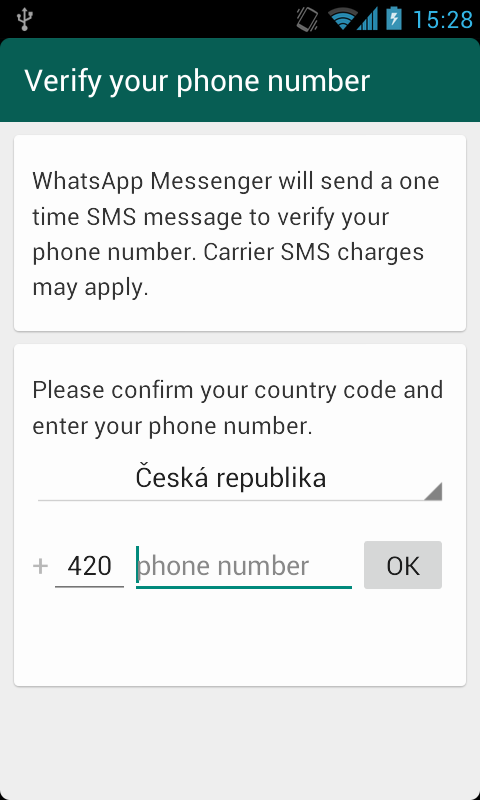
\includegraphics[width=0.4\textwidth]{whatsapp-registration.png}
	\caption{WhatsApp's registration process}
	\label{img:whatsapp_reg}
\end{figure}

Older version of WhatsApp offered an alternative verification process. Instead of the user waiting for a text message, he was rather supposed to send a SMS to one of WhatsApp's phone numbers where he included his email. WhatsApp later sent verification code to the email and user verified himself with this code \cite{whatsapp-shootingthemsg}.

In 2011 research showed this method has serious drawbacks. To hijack user's account attacker first opted for this method. Then using SMS spoofing service\footnote{popsat co to je, nebo není třeba?} he sent SMS to WhatsApp's phone number pretending it originates from the victim. Attacker set the content of the message to an email he owned, leading to WhatsApp sending the verification code to the attacker. The attacker then simply entered the code from an email and successfully hijacked the victim's account \cite{whatsapp-hijack1}.

Following these findings another method to bypass the registration process was published. During the registration phase WhatsApp \footnote{opět přípomínat, že se jedná o starší verzi?} sent a request for the verification SMS to be sent to the client in HTTP request similiar to this: \cite{whatsapp-shootingthemsg}


\begin{lstlisting}[caption={HTTP request to dispatch SMS}]
GET [..]?to=4915143[..]&auth=659&[..]
HTTP/1.1
User-Agent: WhatsApp/2.6.4 iPhone_OS/4.3.3 Device/iPhone_4
\end{lstlisting}

The request contained the final verification code in the GET parameter. That leads to a conclusion the client created the verification code, not the server, and expected user's confirmation. An attacker could simply intercept the request\footnote{Přidat poznámku o HTTP/HTTPS a zachycení requestu?}, retrieved the verification code and made sure the request didn't arrive to WhatsApp's servers to let the victim unaware of malicous intentions.

Attacker then created a fake HTTP OK response to let the messenger think the request was successful and entered retrieved verification code from the intercepted request. The attacker successfully hijacked the victim's WhatsApp identity and can both send and recieve all his messages.


The author of the research notified WhatsApp developers beforehand and WhatsApp fixed this issue before the research was made public \cite{whatsapp-shootingthemsg}.

To the date of writing this thesis WhatsApp client doesn't offer discussed verification method anymore.


\subsubsection{Password generation}

WhatsApp uses lightly modified version of XMPP \cite{whatsapp-xmpp}. During the registration process it creates a username based on the user's phone number. In newer versions of the client the password is generated on server's side \cite{whatsapp-imei}. However, the previous Android versions used the phone's IMEI  number as password \cite{whatsapp-imei}\cite{whatsapp-imei2}.

\begin{lstlisting}[caption={Pseudo-code of password generation on Android}]
md5(revert('IMEI')) 
\end{lstlisting}

Any phone number -- IMEI pair was therefore all an attacker needed to send messages on victim's behalf. Numerous applications are collecting plenty of user data and the IMEI and phone numbers might be among them. For instance any database leak with such information would lead directly to large accounts abuse.

\subsubsection{Messages encryption}

TODO


\subsection{Including Signal's protocol}

On November 18, 2014, Open Whisper Systems, the creators behind Signal messenger, announced a partnership with WhatsApp. The partnership should have escalated into incorporating OWS' encryption protocol to WhatsApp bringing end-to-end encryption to all WhatsApp clients \cite{openwhisperwhatsapp}.

Open Whisper Systems stated: \emph{``we are moving quickly towards a world where all WhatsApp users will get end-to-end encryption by default.''} \cite{openwhisperwhatsapp}

WhatsApp confirmed this partnership, however did not comment it any further nor offered any further information\cite{x}. No additional information from Open Whisper Systems' side had been released as well. Therefore this thesis assumes WhatsApp shares no code base with Signal, since it can't be verified.

\section{Telegram}

Telegram is instant messaging service, enabling users to send messages, photos, videos, stickers and files. It was first released on August 14, 2013\cite{telegramfaq}. Telegram describes itself as fast and secure solution for instant messaging \cite{telegramfaq} and claims to be safer than WhatsApp\cite{telegramfaq}. Compared to WhatsApp, Telegram is more cloud-based, it stores all messages on its servers and sync them with all user's devices \cite{telegramfaq}. 

Similar to WhatsApp user can contact someone by his phone number. Telegram provides classical username approach as well. User needs to know the reciepent's phone number or Telegram username in order to communicate with him.

All clients are licensed under GPLv2 or GPLv3 license, however the server-side part of Telegram is closed-sourced and proprietery. TODO overit

In 2015 Brazilian judiciary ordered WhatsApp to shut down for 48 hours \cite{whatsappbrazil}. During this event, which was finally lowered to only 12 hours, Telegram welcomed 5 million new users \cite{whatsappbrazil}. It may be therefore considered as a direct competitor to WhatsApp.

In September 2015, Telegram officials stated announced it has 60 million active users.\cite{x}


\subsection{Secret chats}

Besides regular chat Telegram provides ``secret chats''. Secret chat messages are encrypted using end-to-end encryption and are not stored on Telegram's servers\cite{telegramfaq}.

\subsection{Cracking Contest}

On November 4, 2014, Telegram published contest with a winning price \$300,000 for cracking its encryption. The contest became quite known in the community and probably provided a bit of advertisiment for Telegram.

The contest remained unsolved until his closure. Number of authors considered it as rigged and stated that the contest does not provide any prove of Telegram's overall security whatsoever.\cite{telegramcontestfail}\cite{telegramcontestfail2}

\subsection{MTProto protocol}

Telegram uses its own encryption protocol called MTProto. One of the basic rules of cryptography is not to ``roll your own crypto''.

TODO popsat celý protokol?


\section{Signal}

Signal is a voice calling and instant messaging application developped by Open Whisper Systems. It was brought to light by merging two applications - the voice calling RedPhone and the text messenger TextSecure both created by the very same company \cite{signalmerge}.

Signal is completely open-sourced including its server side.

TODO

\section{Threema}

Threema is paid proprietary instant messaging application. Users can send  photos, videos, voice messages, QR codes, polls and files \cite{threemahomepage}. TODO: citovani homepage?

It provides end-to-end encryption and claims to prevent collection of any metadata \cite{threemahomepage}.

Threema does not use phone numbers or usernames. It generates a random ID for user identification. Phone number and email are not required, no personal information are therefore needed.

As of June 2015, Threema had 3.5 million active users, mostly in german-speaking countries.\cite{threemausers}

\section{WeChat}

WeChat is properietary application. It was released in January 2011 and allows users to send text messages, voice messages, communicate via phone or video calls, it provides location sharing functions and other various functions \cite{wechatfeatures}.

As of August 2015, WeChat has 600 million active users, vast majority of them located in China.\cite{wechatusers}

\begin{conclusion}

Zaver TODO


\begin{itemize}
	\item The algorithm assigns code to each source unit irrespective to its position (statistical compression methods).
	\item The Markov's model of $n$-th order look at previous $n$ source units to assign code. The simplist of this codes, 0th order, are mentioned above.
	\item The models based on finite automata.
\end{itemize}

	

\end{conclusion}

\bibliographystyle{iso690}
\bibliography{ref}

\appendix

% \printglossaries

\chapter{Contents of CD}\label{app:CDcontent}

Visualise the contents of enclosed media. Use of \verb|dirtree| is recommended. Note that directories src and text with appropriate contents are mandatory.


\begin{figure}
	\dirtree{%
		.1 readme.txt\DTcomment{the file with CD contents description}.
		.1 data\DTcomment{the data files directory}.
		.2 graphs\DTcomment{the directory of graphs of experiments}.
		.3 *.eps\DTcomment{the B/W graphs}.
		.3 *.png\DTcomment{the color graphs}.
		.3 *.dat\DTcomment{the graphs data files}.
		.1 exe\DTcomment{the directory with executable WBDCM program}.
		.2 wbdcm\DTcomment{the WBDCM program executable (UNIX)}.
		.2 wbdcm.exe\DTcomment{the WBDCM program executable (Windows)}.
		.1 src\DTcomment{the directory of source codes}.
		.2 wbdcm\DTcomment{the directory of WBDCM program}.
		.3 Makefile\DTcomment{the makefile of WBDCM program (UNIX)}.
		.2 thesis\DTcomment{the directory of \LaTeX{} source codes of the thesis}.
		.3 figures\DTcomment{the thesis figures directory}.
		.3 *.tex\DTcomment{the \LaTeX{} source code files of the thesis}.
		.1 text\DTcomment{the thesis text directory}.
		.2 thesis.pdf\DTcomment{the Diploma thesis in PDF format}.
		.2 thesis.ps\DTcomment{the Diploma thesis in PS format}.
	}
\end{figure}


\end{document}
